\documentclass[a4paper,14pt]{extarticle}

\usepackage[top=1in, bottom=1in, left=1in, right=1in]{geometry}
\usepackage[utf8]{inputenc}
\usepackage[russian]{babel}
\usepackage[final]{graphicx}
\usepackage{caption}
\usepackage{subcaption}
\usepackage{chngcntr}
\usepackage{amsmath}
\usepackage{amsfonts}
\usepackage{pgfplots}
\usepackage{pgfplotstable}
\usepgfplotslibrary{fillbetween}
\usepackage{float}
\usepackage{lipsum}% http://ctan.org/pkg/lipsum
\usepackage{multicol}% http://ctan.org/pkg/multicol
\usepackage{hhline}
\usepackage{tabularx}
\usepackage{tikz,xcolor}
\usepackage{tkz-graph}
\usepackage{float}
\usepackage{mathtools}
\usepackage{todonotes}
\usepackage{listings}
\usepackage{epstopdf}
\usepackage{epsfig}
\usepackage[makeroom]{cancel}
\usepackage{subcaption}

\usetikzlibrary{arrows, petri, topaths}

\counterwithin{figure}{section}
\counterwithin{equation}{section}
\counterwithin{table}{section}

\DeclareMathOperator*{\argmin}{arg\,min}
\DeclareMathOperator*{\argmax}{arg\,max}
\DeclareMathOperator{\sinc}{sinc}

\definecolor{mygreen}{RGB}{28,172,0} % color values Red, Green, Blue
\definecolor{mylilas}{RGB}{170,55,241}

\lstset{language=Matlab,%
  %  basicstyle=\color{red},
    breaklines=true,%
    morekeywords={matlab2tikz,ylim,xlim,square,ones,double},
    keywordstyle=\color{blue},%
    morekeywords=[2]{1}, keywordstyle=[2]{\color{black}},
    identifierstyle=\color{black},%
    stringstyle=\color{mylilas},
    commentstyle=\color{mygreen},%
    showstringspaces=false,%without this there will be a symbol in the places where there is a space
    numbers=left,%
    numberstyle={ \color{black}},% size of the numbers
    numbersep=15pt, % this defines how far the numbers are from the text
    emph=[1]{for,end,break,switch,case,otherwise},emphstyle=[1]\color{red}, %some words to emphasise
    %emph=[2]{word1,word2}, emphstyle=[2]{style},    
}


\begin{document}
\begin{titlepage}
\centering 
{\bfseries Санкт-Петербургский Политехнический Университет} \\
Институт компьютерных наук и технологий \\
Кафедра компьютерных систем и программных технологий \\
\vspace{5cm}
{\centering \textbf{Отчёт по лабораторной работам №4 и №5} \\ 
\vspace{0.15cm}
\textbf{Дисциплина}: Телекоммуникационные технологии \\
\vspace{0.15cm}
\textbf{Тема}: Аналоговая модуляция. Фазовая и частотная модуляция.} \\
\vspace{4cm}
\hfill {\bfseries Работу выполнил студент}  \\
\hfill гр. 33501/4 Леженин Ю.И. \\
\hfill {\bfseries Преподаватель}  \\
\hfill Богач Н.В.
\vfill
Санкт-Петербург \\
{\large \today\par}
\end{titlepage}

\section{Цель работы.}

Изучение амплитудной модуляции/демодуляции сигнала. Изучение частотной и фазовой модуляции/демодуляции сигнала.

\section{Постановка задачи.} 

Сгенерировать однотональный сигнал низкой частоты. Выполнить амплитудную модуляцию/демодуляцию для различных значений глубины модуляции, амплитудную модуляцию/демодуляцию с подавлением несущей, однополосную модуляцию и синхронное детектирование. Выполнить фазовую и частотную модуляцию/демодуляцию. Получить спектры модулированных сигналов.


\section{Ход работы.}

\subsection{Амплитудная модуляция.}

Амплитудно-модулированный сигнал задается по закону
\begin{multline*}
u(t) = U_m \, [1 + M \, \cos(\Omega\,t)] \, \cos(\omega_0\,t) = \\
 = U_m \, \big[ cos(\omega_0\,t) + \frac{M}{2}\,cos((\omega_0 + \Omega)\,t) + \frac{M}{2}\,\cos((\omega_0 -\Omega)\,t)\big],
\end{multline*}
где $M$ -- глубина модуляции, $\Omega$ -- частота модулируемого сигнала, $\omega_0$ -- несущая частота. 

%Для демодуляции выполняется синхронное детектирование, полученный сигнал умножается на гармонику с несущей частотой:
%\begin{multline*}
%y(t) = U_m \, [1 + M \, \cos(\Omega\,t)] \, \cos(\omega_0\,t) \, \cos(\omega_0\,t) = \\
% = \frac{U_m}{2} (1 + M\,\cos(\Omega\,t) + \cos(2\,\omega_0\,t) + M\,\cos(\Omega\,t)\,\cos(2\,\omega_0\,t).
%\end{multline*}
%Выделение информационной составляющей выполняется с помощью низкочастотной фильтрации.

Для повышения КПД используется балансная модуляция:
\begin{equation*}
u(t) = U_m \, \cos(\Omega\,t) \, \cos(\omega_0\,t).
\end{equation*}
Однако отсутствие опорного сигнала с несущей частотой значительно усложняет демодуляцию. 

Кроме того, ввиду идентичности информации на частотах ниже и выше несущей, может выполнятся однополосная амплитудная модуляция:
\begin{equation*}
u(t) = U_m \, M \, \cos((\omega_w \pm \Omega) \, t).
\end{equation*} 

Для демонстрации амплитудной модуляции был сгенерирован однотональный сигнал, для которого была выполнена модуляция при $M = 1$, $M = 0.5$, модуляция с подавлением несущей и однополосная модуляция. Результаты представлены на рисунках \ref{am1}, \ref{am2}, \ref{am3}, \ref{am4}.

\begin{figure}[p]
\centering
%\begin{subfigure}[b]{1\textwidth}
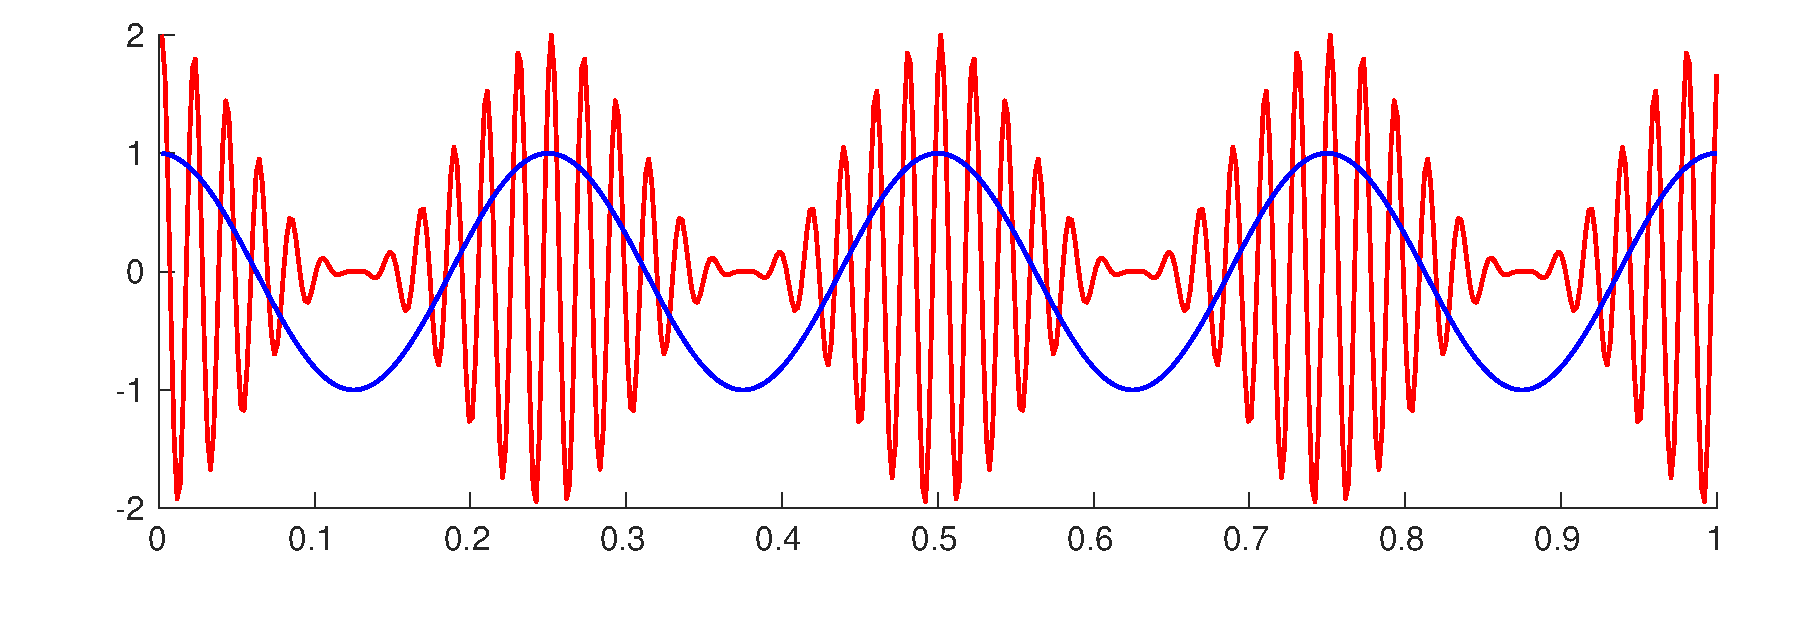
\includegraphics[width=1\textwidth]{ammod_m1.eps}
%\caption{}
%\end{subfigure}
%\begin{subfigure}[b]{1\textwidth}
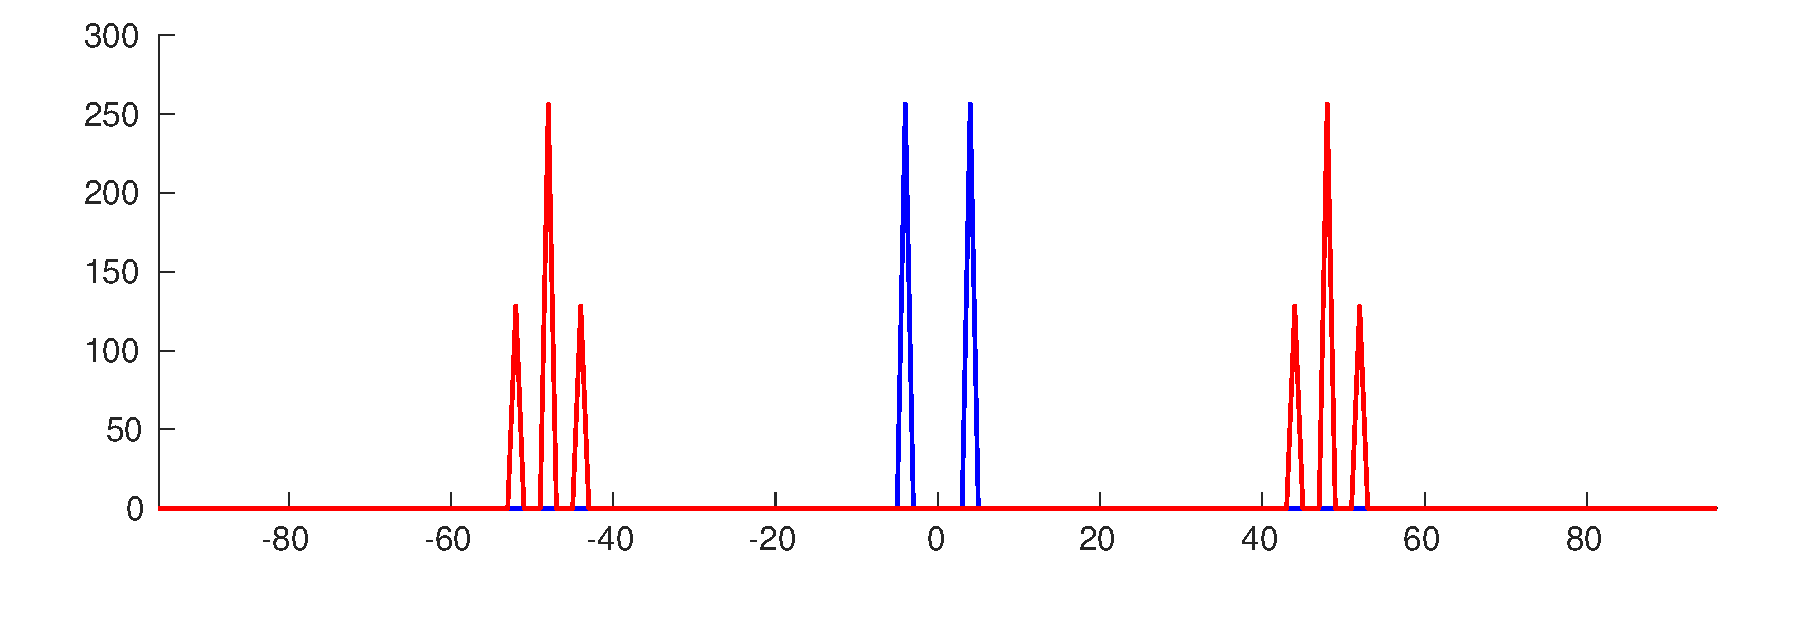
\includegraphics[width=1\textwidth]{ammod_s_m1.eps}
%\caption{}
%\end{subfigure}
%\begin{subfigure}[b]{1\textwidth}
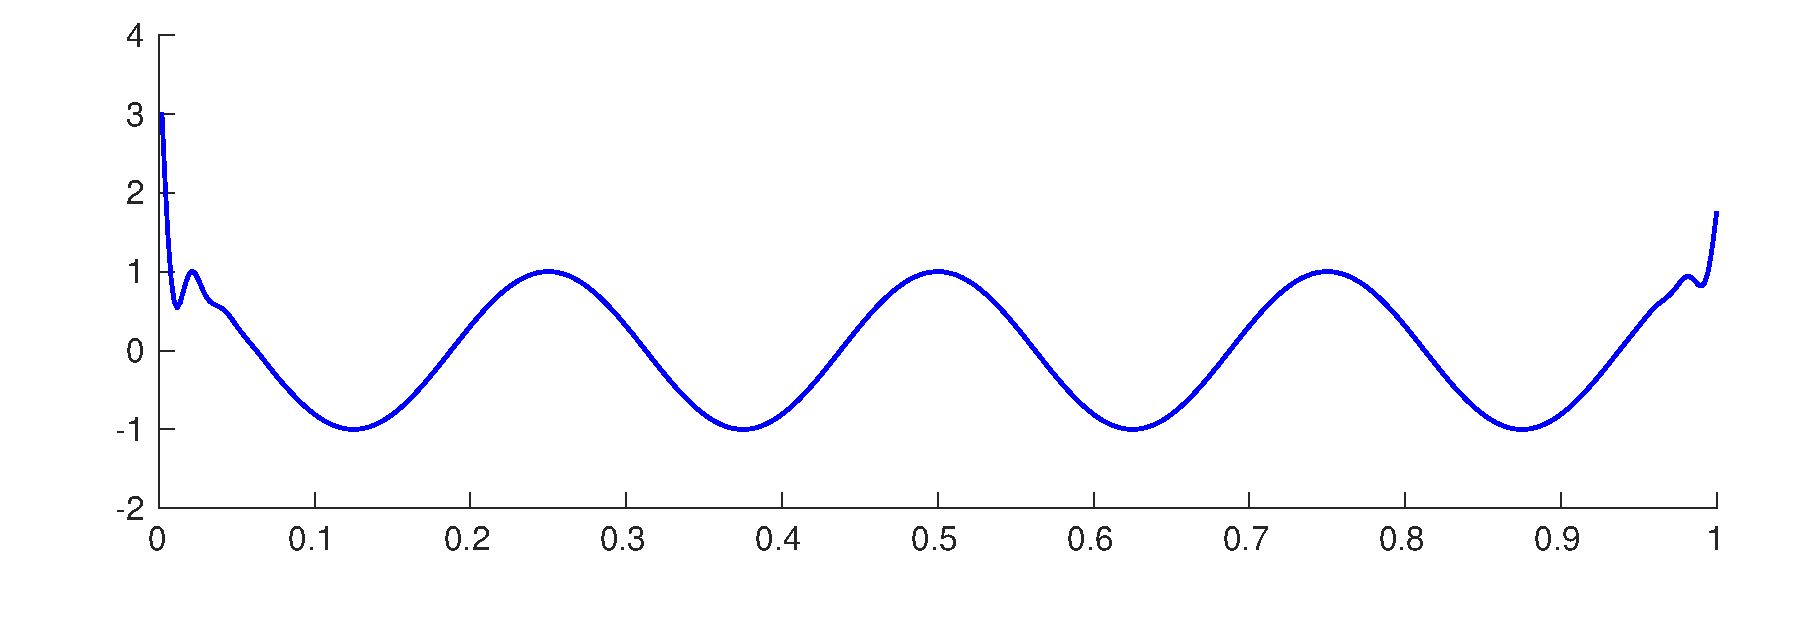
\includegraphics[width=1\textwidth]{amdemod_m1.eps}
%\caption{}
%\end{subfigure}
\captionsetup{justification=centering,margin=0.5cm}
\caption{Модулируемый однотональный сигнал ($\Omega = 4$ Гц), амплитудно-модулированный сигнал ($\omega_0 = 64$ Гц, $M = 1$), их спектры, демодулированный сигнал.}
\label{am1}
\end{figure}


\begin{figure}[p]
\centering
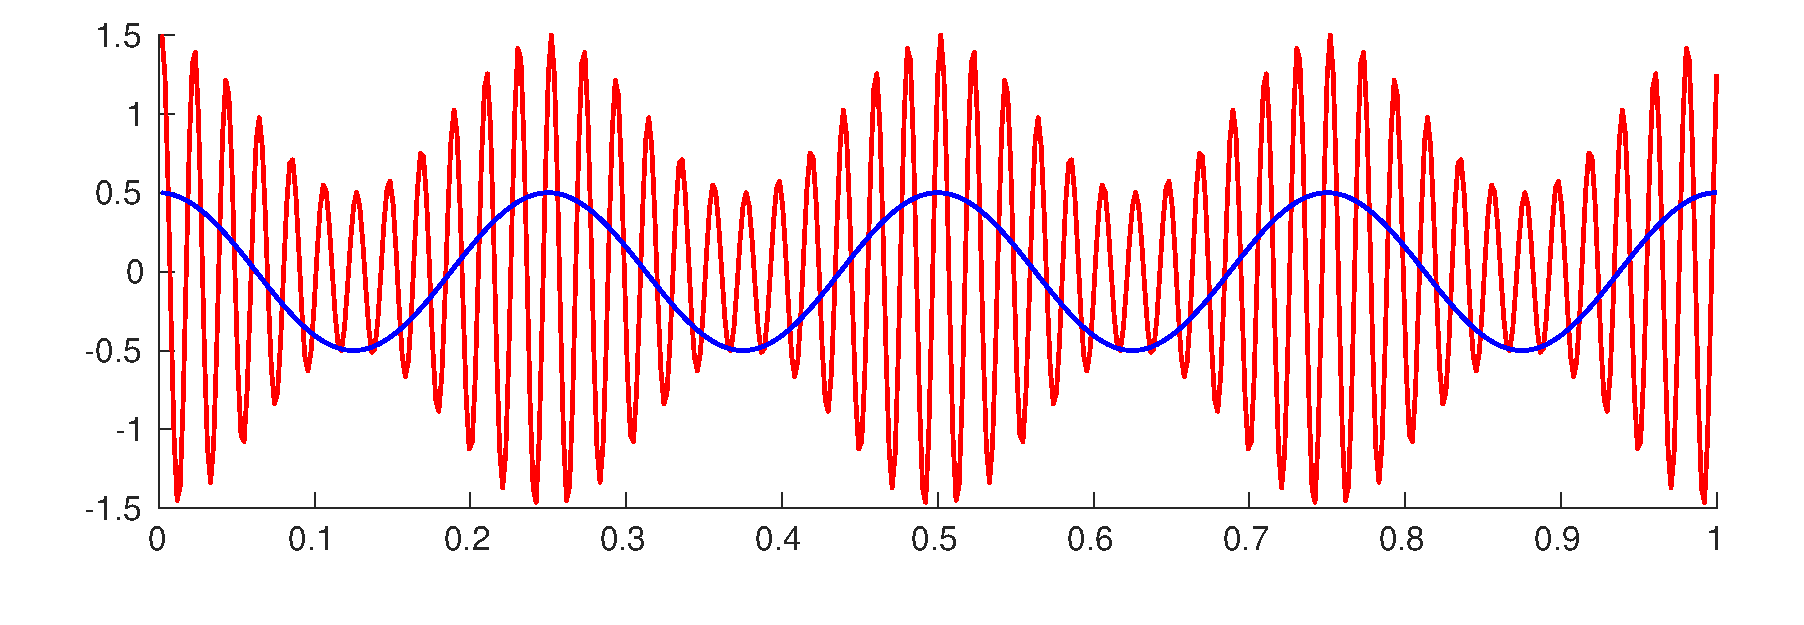
\includegraphics[width=1\textwidth]{ammod_m05.eps}
\includegraphics[width=1\textwidth]{ammod_s_m05.eps}
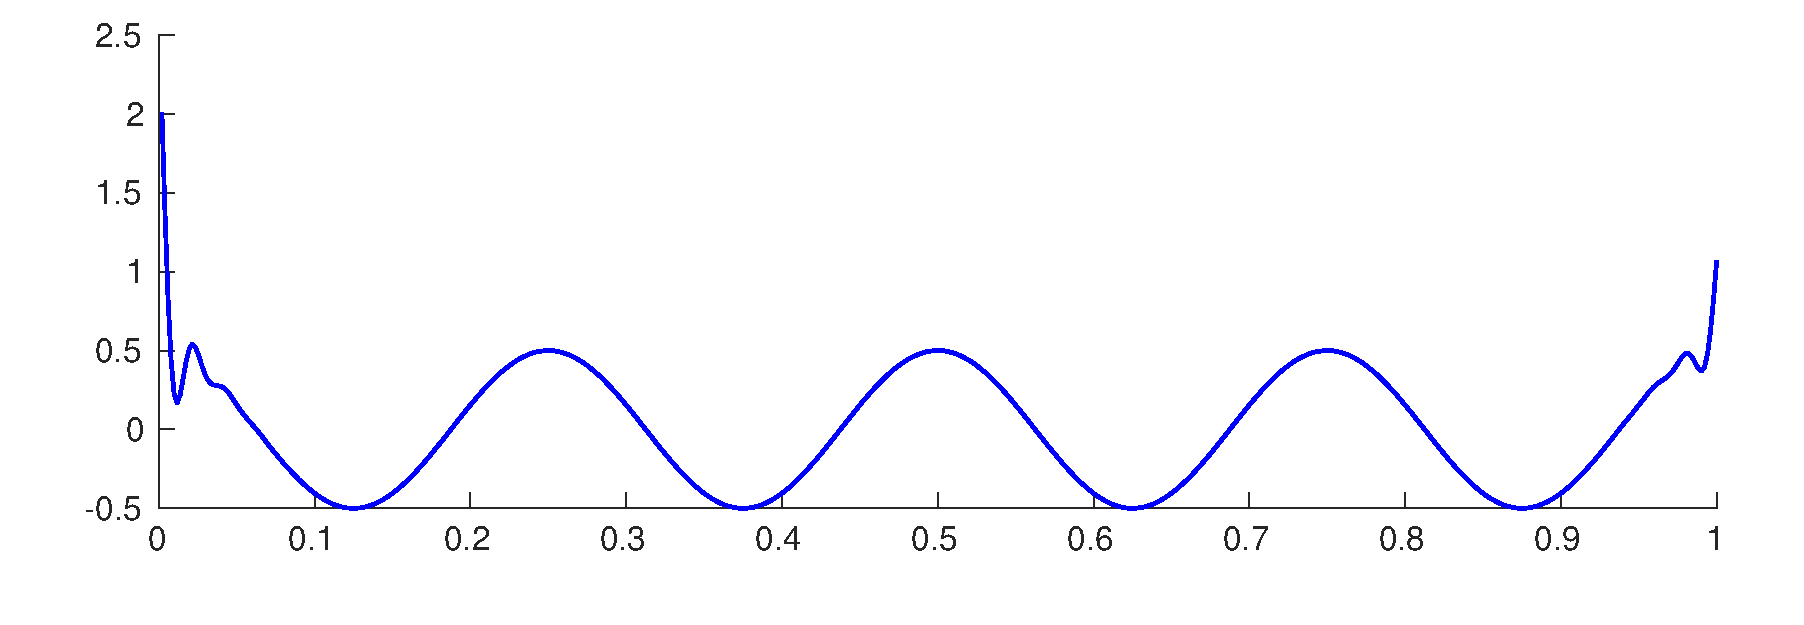
\includegraphics[width=1\textwidth]{amdemod_m_05.eps}
\captionsetup{justification=centering,margin=0.5cm}
\caption{Модулируемый однотональный сигнал ($\Omega = 4$ Гц), амплитудно-модулированный сигнал ($\omega_0 = 64$ Гц, $M = 0.5$), их спектры, демодулированный сигнал.}
\label{am2}
\end{figure}

\begin{figure}[p]
\centering
\includegraphics[width=1\textwidth]{ammod_m_inf.eps}
\includegraphics[width=1\textwidth]{ammod_s_m_inf.eps}
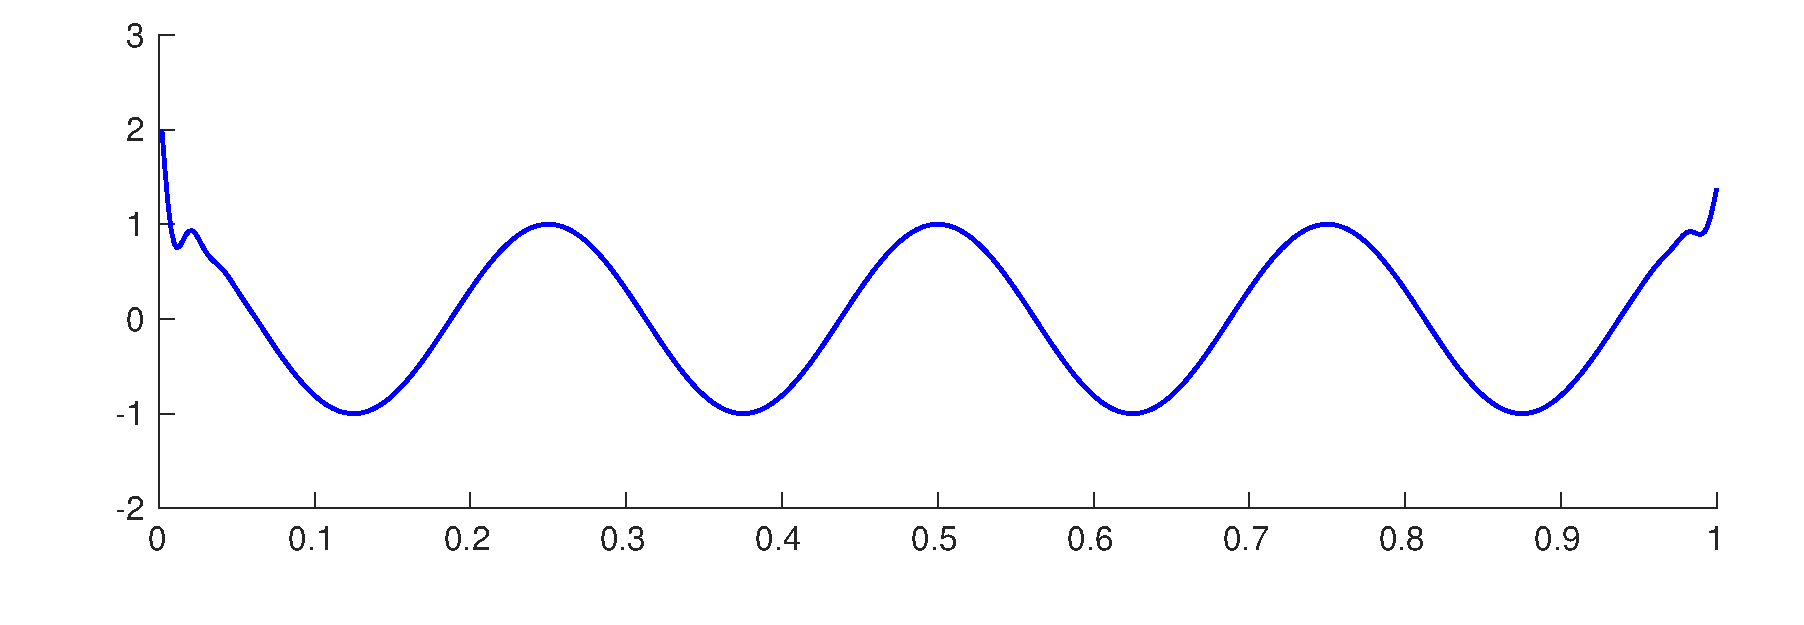
\includegraphics[width=1\textwidth]{amdemod_m_inf.eps}
\captionsetup{justification=centering,margin=0.5cm}
\caption{Модулируемый однотональный сигнал ($\Omega = 4$ Гц), амплитудно-модулированный сигнал ($\omega_0 = 64$ Гц) с подавлением несущей, их спектры, демодулированный сигнал.}
\label{am3}
\end{figure}

\begin{figure}[p]
\centering
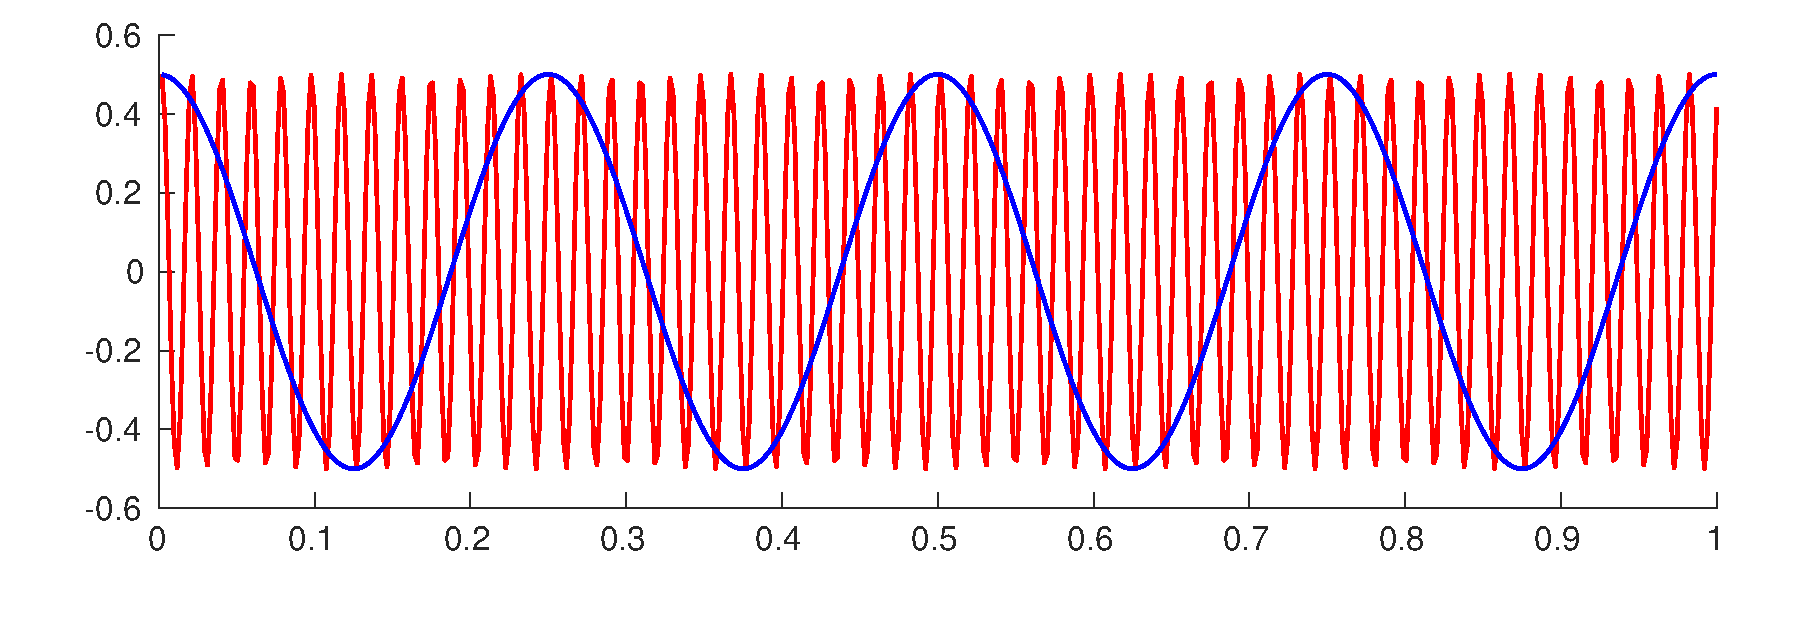
\includegraphics[width=1\textwidth]{ssbmod.eps}
\includegraphics[width=1\textwidth]{ssbmod_s.eps}
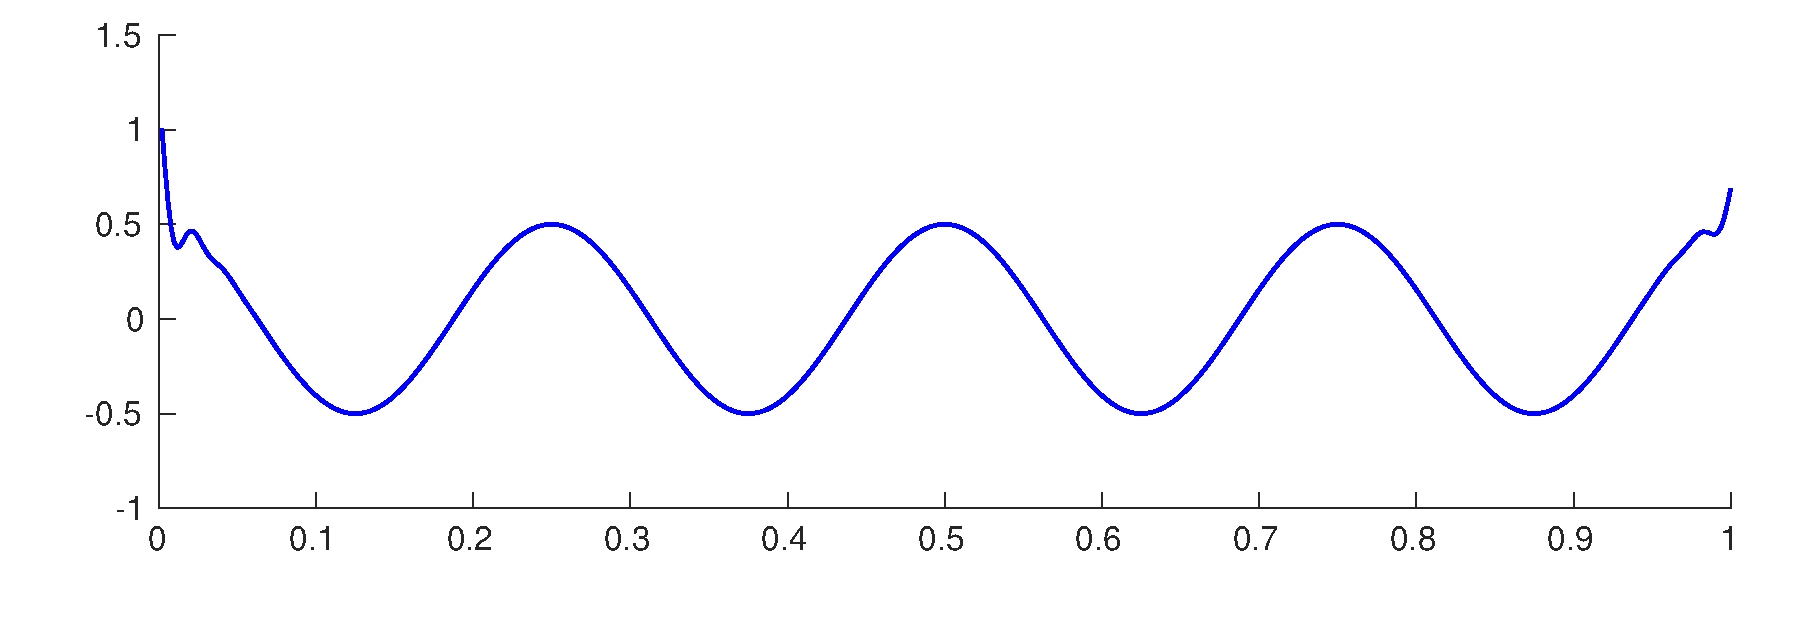
\includegraphics[width=1\textwidth]{ssbdemod_s.eps}
\captionsetup{justification=centering,margin=0.5cm}
\caption{Модулируемый однотональный сигнал ($\Omega = 4$ Гц), однополосный амплитудно-модулированный сигнал ($\omega_0 = 64$ Гц) с подавлением несущей, их спектры, демодулированный сигнал.}
\label{am4}
\end{figure}

\subsection{Частотная и фазовая модуляция.}

При фазовой модуляции фаза модулированного сигнала пропорциональна амплитуде передаваемого сигнала:
\begin{equation*}
u(t) = U_m \, \cos(\omega_0 \, t + k \, s(t)).
\end{equation*}
При этом полная фаза колебаний задается выражением
\begin{equation*}
\psi(t) = \omega_0 \, t + k \, s(t).
\end{equation*}
Девиация фазы вниз и вверх определяется следующим образом:
\begin{equation*}
\Delta \phi_\text{в} = k s_{max}, ~ ~ ~ \Delta \phi_\text{н} = k s_{min}.
\end{equation*} 
Мгновенная частота является производной от полной фазы:
\begin{equation*}
\omega(t) = \frac{d}{dt} \psi(t) =  \omega_0 + k \cdot \frac{d}{dt} s(t).
\end{equation*}
Видно, что при фазовой модуляции частота модулированного сигнала зависит от производной модулируемого сигнала. 

При фазовой модуляции фаза модулированного сигнала пропорциональна интегралу передаваемого сигнала:
\begin{equation*}
u(t) = U_m \, \cos(\omega_0 \, t + k \int_0^t s(t) dt).
\end{equation*}
При этом полная фаза колебаний определяется как
\begin{equation*}
\psi(t) = \omega_0 \, t + k \, \int_0^t s(t) dt,
\end{equation*}
а мгновенная частота
\begin{equation*}
\omega(t) = \frac{d}{dt} \psi(t) =  \omega_0 + k \cdot s(t).
\end{equation*}
Девиация частоты вниз и вверх находится следующим образом:
\begin{equation*}
\Delta \omega_\text{в} = k s_{max}, ~ ~ ~ \Delta \omega_\text{н} = k s_{min}.
\end{equation*} 
Частота модулированного сигнала зависит от амплитуды модулируемого сигнала.

\begin{figure}[p]
\centering
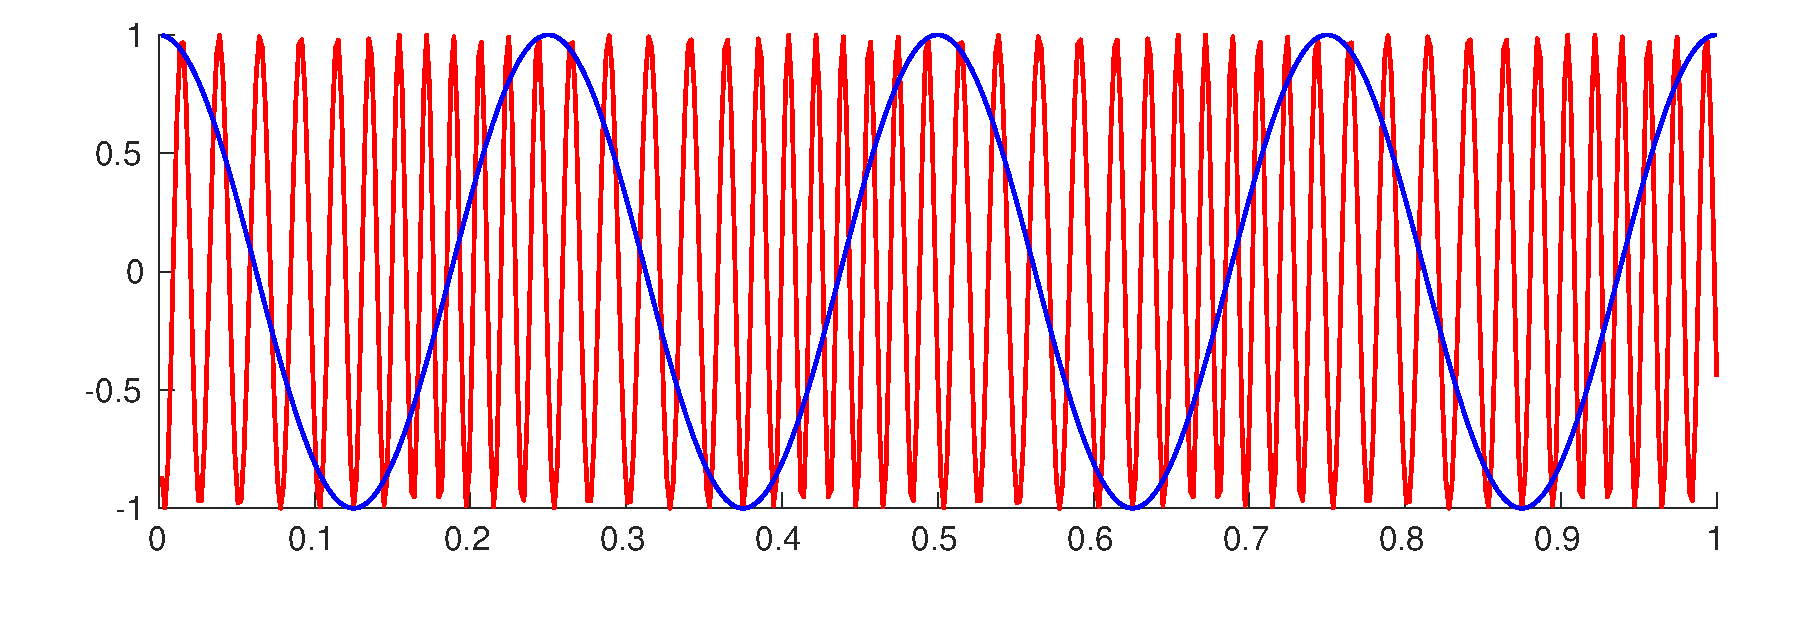
\includegraphics[width=1\textwidth]{pmod.eps}
\includegraphics[width=1\textwidth]{pmod_s.eps}
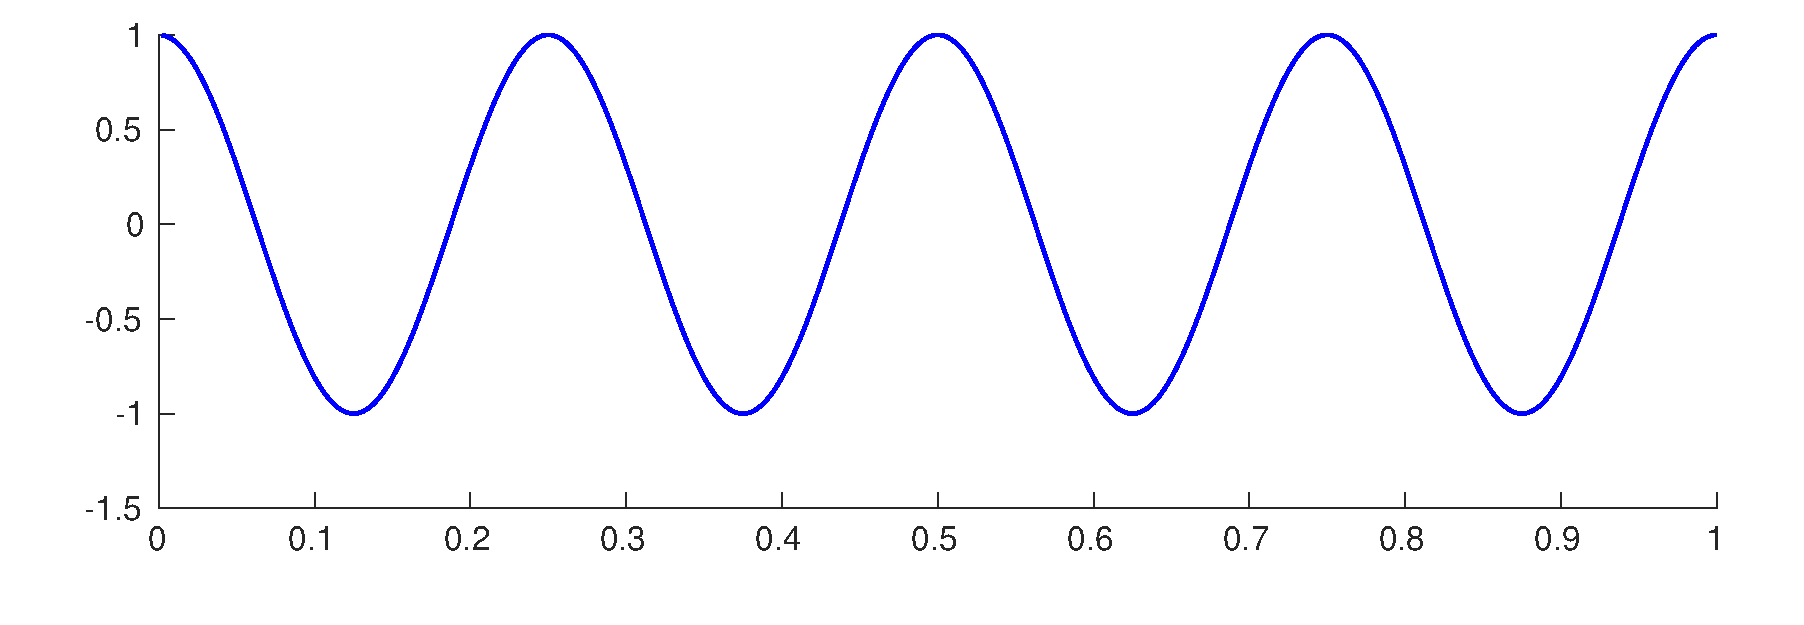
\includegraphics[width=1\textwidth]{pdemod.eps}
\captionsetup{justification=centering,margin=0.5cm}
\caption{Модулируемый однотональный сигнал ($\Omega = 4$ Гц), фазово-модулированный сигнал ($\omega_0 = 48$ Гц, $\Delta \phi = \frac{5\,\pi}{6}$), их спектры, демодулированный сигнал.}
\label{pm}
\end{figure}

\begin{figure}[p]
\centering
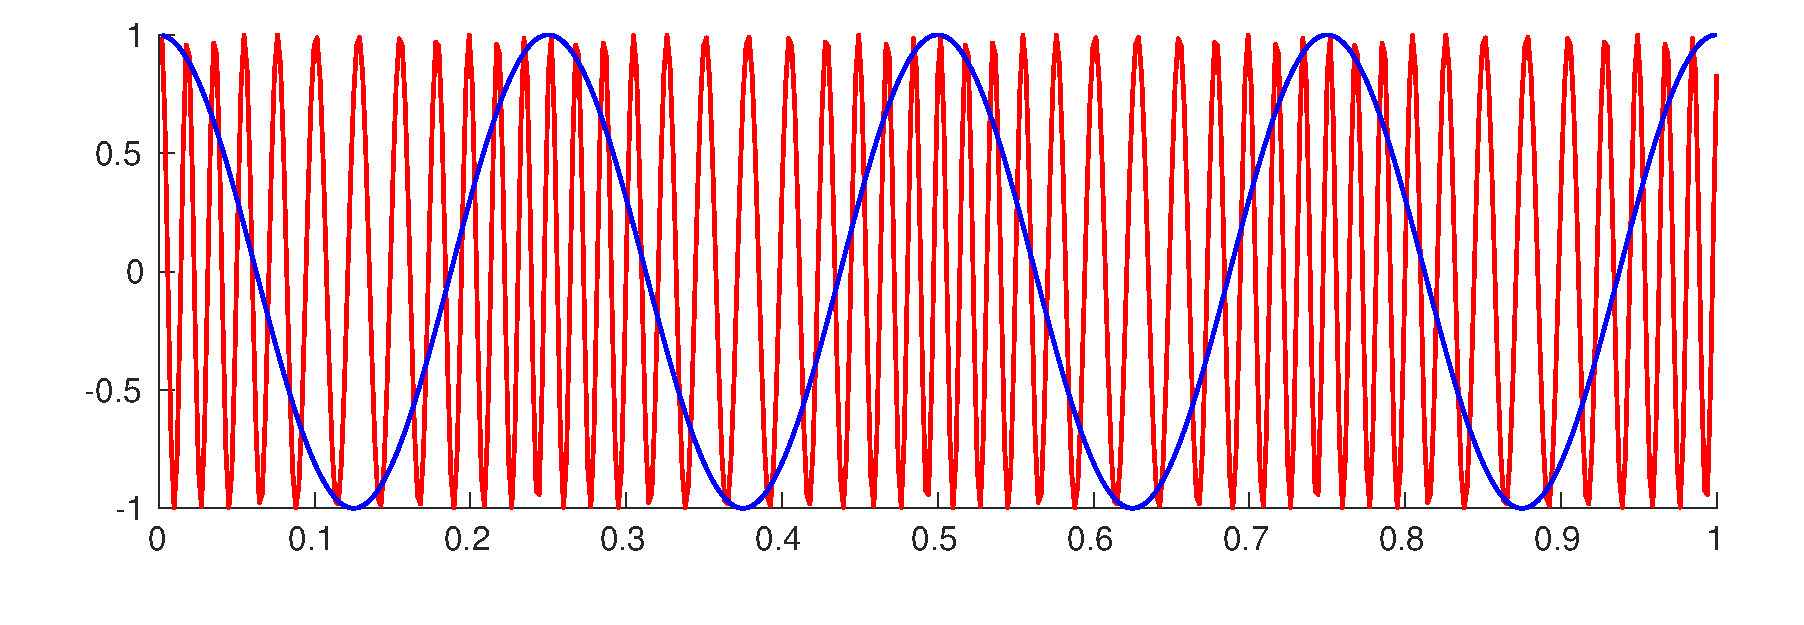
\includegraphics[width=1\textwidth]{fmod.eps}
\includegraphics[width=1\textwidth]{fmod_s.eps}
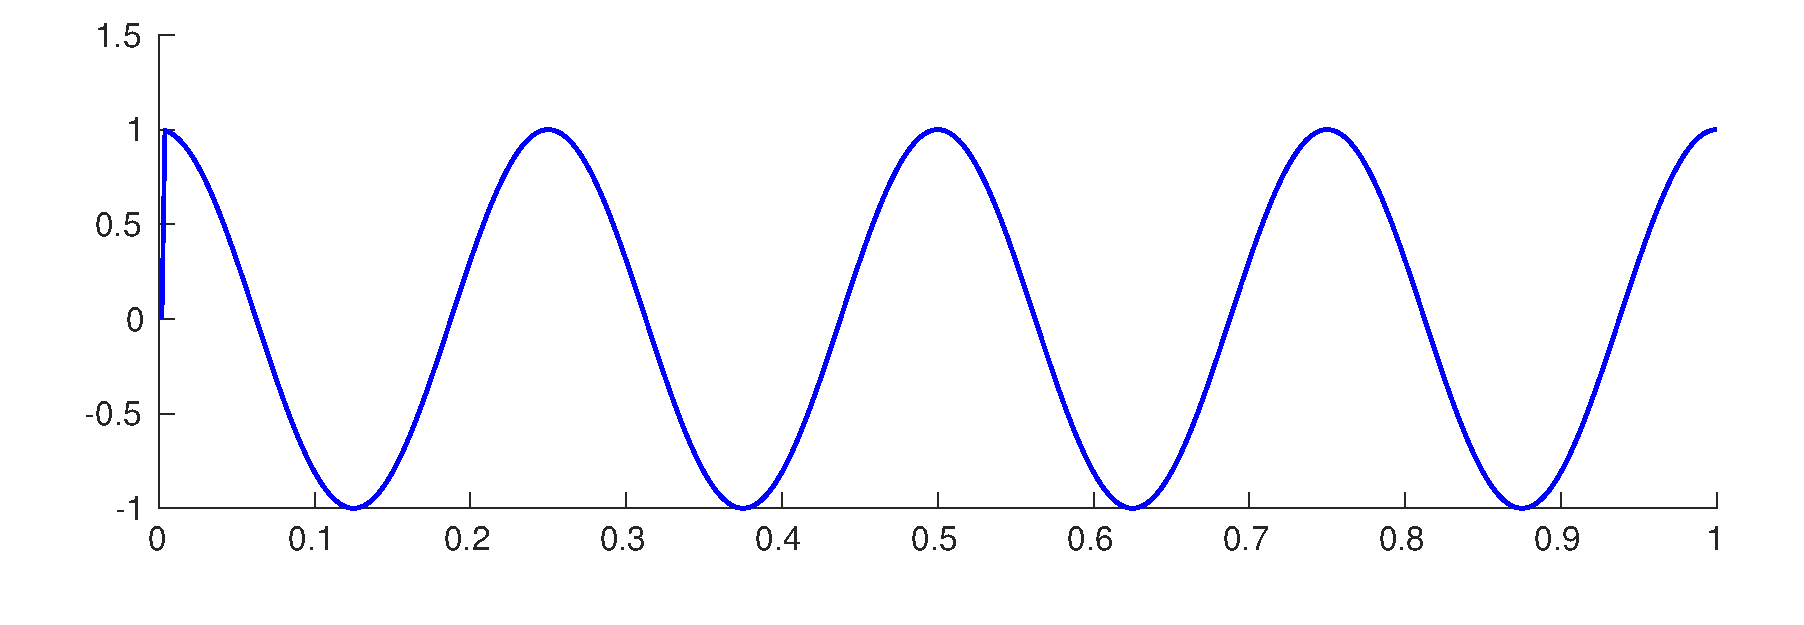
\includegraphics[width=1\textwidth]{fdemod.eps}
\captionsetup{justification=centering,margin=0.5cm}
\caption{Модулируемый однотональный сигнал ($\Omega = 4$ Гц), частотно-модулированный сигнал ($\omega_0 = 48$ Гц, $\Delta \omega = 12$ Гц), их спектры, демодулированный сигнал.}
\label{fm}
\end{figure}

\section{Выводы.}

Модуляция позволяет перенести информацию содержащуюся в одном сигнале на другой сигнал, обладающими необходимыми свойствами. Модуляция дает возможность перенести спектр сигнала на заданный диапозон частот и выполнить частотное разделение каналов, что позволяет более эффективно использовать передающее оборудование.

Как правило, для модуляции используют гармонические колебания. В зависимости от того, на какой из параметров переносится информация, различают амплитудную (АМ), частотную (ЧМ) или фазовую (ФМ) модуляцию несущего сигнала.

Фазовая и частотная модуляции позволяют расширить спектра сигнала и тем самым повысить помехоустойчивость передачи.


\section{Приложение.}

\lstinputlisting[frame=single, caption=Программа для выполнения амплитудной модуляции/демодуляции.]{lab4_script.m}

\lstinputlisting[frame=single, caption=Программа для выполнения частотной и фазовой модуляции/демодуляции.]{lab5_script.m}


\end{document}